\chapter{EMPIRICAL EVALUATION}
\label{chapter:empevaluation}
In this section, we describe our settings in Section~\ref{sec:settings}, followed by research questions in Section~\ref{sec:rqs}. Finally, we discuss experiment results in Section~\ref{sec:results}

\section{Experiment Settings}
\label{sec:settings}
We collected a dataset of 100 GitHub projects described in Section~\ref{sec:datacollection}. For performance commit identification and code change analysis, we use a computer with 2.4 GHz Intel Core i7 CPU with 16GB of Memory, and Ubuntu 14.10 LTS operating system. 

\section{Research Questions}
\label{sec:rqs}
In our analysis, we seek to answer following research questions. 

\begin{itemize}
	\item \textbf{RQ1:} What are the major root causes of \unity performance bugs?
	
	\item \textbf{RQ2:} What are the most common performance bug prone methods of \unity performance bugs?
	
	\item \textbf{RQ3:} How difficult is to fix \unity performance bugs?
	
	\item \textbf{RQ4:} Which files are common to resolve \unity performance bugs?
\end{itemize}


\section{Results}
\label{sec:results}

\subsection{RQ1:Root Causes of Unity Performance Bugs}
\label{subsec:rootcause}
With detailed root cause analysis, we identified Unity's performance bug fix taxonomy. That means, we categorized the bugs depending on their types and how they got fixed. We classified these 230 bugs into 15 categories. Figure~\ref{figure:rq1category} shows the Unity performance bug taxonomy with their frequency. Among these 230 performance  bugs, largest category is Asset/Prefab related optimization. In Unity game components are stored in asset file and for reusability some assets are  bundled together and used as prefab file. 18 fixes are related to loop optimization and 16 fixes are related to caching related fix. Data Structure related performance fixes accounts for 16 cases. Other fixes are: Don't use var, avoid linq and regx, string operation, use of readonly and constant, Memory cleanup, move unnecessary code, Run code in every X frame and thread related fixes. Performance fixes that we cannot generalized are considered as Others type. 


\begin{figure*}[t]
	%%\vspace{-0.2cm}
	\centering
	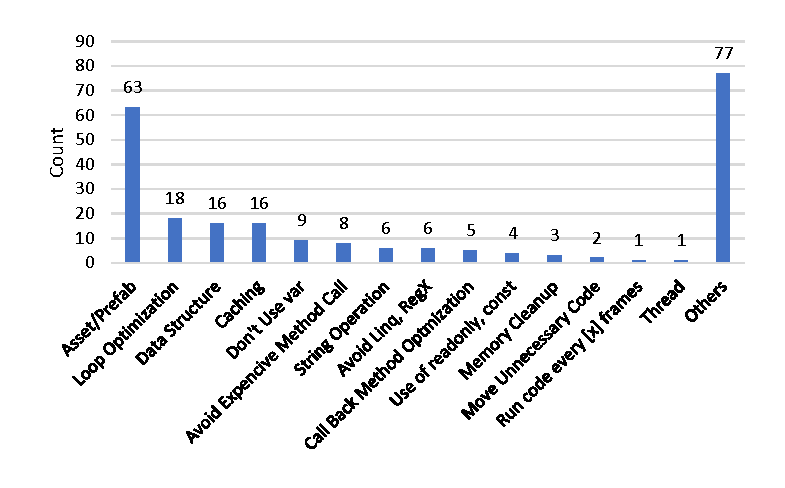
\includegraphics[width=0.8\textwidth]{figure/rq1_taxonomy.eps}
	%\vspace{-0.3cm}
	\caption{Unity Performance Bug Taxonomy with Frequency}
	%	\vspace{-0.3cm}	
	\label{figure:rq1category}
\end{figure*}

In the following subsections, we will discuss detail about each of the bug category.

\subsubsection{Asset/Prefab Bug Fix}
The graphical parts of the game can primarily impact two computer systems: the GPU and the CPU. Considering that, a major portion of Unity Performance bugs are related to Asset or Prefab optimization. Example~\ref{example:taxonomy1} shows such an example of a performance bug fix. In this fix, developers improved performance prefab that is bundling related components as a bundle. We check the unity documentation too that uses of prefab are helpful for performance improvement.

\begin{example}
	\begin{lstlisting}[escapechar=!]	
	!\colorbox{light-green}{+\-\-\- \!u\!1001 \& 1246218760}!  
	!\colorbox{light-green}{+Prefab:}! 
	!\colorbox{light-green}{+         m\_ObjectHideFlags: 0}! 
	!\colorbox{light-green}{+         serializedVersion: 2}! 
	!\colorbox{light-green}{+     		m\_Modification:}! 
	!\colorbox{light-green}{+				m\_TransformParent: {fileID: 713704410}}!      
	\end{lstlisting}
	\caption{Asset/Prefab Related Fix
		\scriptsize{\textit{(AdrianBZG/Medieval\_Warfare\_VR\-Unity:207bc51)}}}
	\label{example:taxonomy1}	
\end{example}
 
\subsubsection{Loop Optimization}
In \unity use of typical "for" loop instead of "foreach" helps to improve performance. We also check several Stackoverflow issues to confirm this fix. So, for Unity it's suggested to use "for" rather than foreach.



\begin{example}
\begin{lstlisting}[escapechar=!]
!\hlp{- foreach (VRTK\_BasicTeleport teleporter in VRTK\_ObjectCache.registeredTeleporters)}!   
!\hlg{+ for (int i = 0; i < VRTK\_ObjectCache.registeredTeleporters.Count; i++)}! 
{
!\hlg{+VRTK\_BasicTeleport teleporter = VRTK\_ObjectCache.registeredTeleporters[i]; }!
teleporter.Teleporting -= new TeleportEventHandler(OnTeleporting);
\end{lstlisting}
  \caption{Loop Optimization
  	\scriptsize{\textit{(gpvigano/VRTK-GearVR-Test:c2c9e08)}}}
  \label{example:diff}  
\end{example}


\subsubsection{Caching-Based Performance Fix}
Caching is the process of storing data in memory or data structure. In Example~\ref{example:caching}, rather than loading gameobject again and again. Dictionary is used to save a copy of the already loaded gameobject. This works as a singleton pattern if not created, then create otherwise return existing instance. Caching is widely used in performance optimization of Unity applications. 

\begin{example}
\begin{lstlisting}[escapechar=!]
!\hlg{+private static Dictionary<string, GameObject> objects = new Dictionary<string, GameObject>();}!
...
!\hlg{+    GameObject FastResource(string resource) \{ }!
!\hlg{+        if (\!objects.ContainsKey(resource)) \{}!
!\hlg{+            objects.Add(resource, (GameObject) Resources.Load(resource));}!
!\hlg{+        \}}!
!\hlg{+        return objects[resource];}!
!\hlg{+ \}}!
...
GameObject CreateFace(Vector3 localPosition, Vector3 scale, Vector3 angles, string type){
...
!\hlp{-        var frontSide = (GameObject)GameObject.Instantiate(Resources.Load(type));}!
!\hlg{+        var frontSide = (GameObject)GameObject.Instantiate(FastResource(type));}!
}
\end{lstlisting}
  \caption{Caching-based Performance Fix
  	\scriptsize{\textit{(stefaanvermassen/virtual-museum-app:b3823da)}}}
  \label{example:caching}  
\end{example}


\subsubsection{Data Structure Related Fix}
The data structure is a particular way of storing data in a computer. Developers must choose the appropriate data structure for better performance. Example~\ref{example:dt} shows a performance fix using right Data Structure. Since this data structure code is always using the first element, so, rather than using a list, the LinkedList is much more effective to get the first item. We got similar issues like using Maps where required.


\begin{example}
\begin{lstlisting}[escapechar=!]
!\hlp{-     private List<GazeSample> stabilitySamples = new List<GazeSample>();}!
!\hlg{+     private LinkedList<GazeSample> stabilitySamples = new LinkedList<GazeSample>();}!
...

!\hlp{- if (stabilitySamples.Count >= StoredStabilitySamples)}!
!\hlg{+                // Remove from front items if we exceed stored samples.}!
!\hlg{+                while (stabilitySamples.Count >= StoredStabilitySamples)}!
					   {
!\hlp{-                    stabilitySamples.RemoveAt(0);}!
!\hlg{+                    stabilitySamples.RemoveFirst();}!
          				}
\end{lstlisting}
  \caption{Data Structure Related Performance Fix
  	\scriptsize{\textit{(stefaanvermassen/virtual-museum-app:b3823da)}}}
  \label{example:dt}  
\end{example}


\subsubsection{Don't Use Var}
It indicates that it is better to use concrete data type rather than using generic data type var. If the compiler cannot determine exact type of type data pointing to var, then it might create compilation error. Apart from that run time type determination might have performance overhead.


\subsubsection{Avoid expensive method call}
There are some methods that are considered as expensive by the developers, such as GetComponent. In Unity, it is common is to call GetComponent to access components. In many cases, developers call GetComponent method inside Update callback to extract components and pass it other methods as parameter. To improve the performance, we can extract all the components in Start callback and reuse the components. This will reduce the repitative GetComponent method call.

\subsubsection{Avoid Linq, Regx}
LINQ is a structured query syntax built in C\# to retrieve data from different types of data sources. Regx represents regular expressions. It is suggested to avoid Linq and regx.  

\subsubsection{String Operation}
For string concatenation, string boxing, we had to use string builder rather than string append function. In C\#, Strings are immutable, which means that after creation if the value is changed it allocate new memory space. Repetitive String value update, concatenation creates lot of garbage. To improve the performance, we should cut down on unnecessary string creation and manipulation. If String value is determined during runtime, it's better to use StringBuilder class. Similarly, we should avoid boxing such as String.Format() method that takes a String and an object parameter. Boxing creates garbage because of what happens behind the scenes. When a value-typed variable is boxed, Unity creates a temporary System.Object on the heap to wrap the value-typed variable. Boxing might create unnecessary memory overhead.


\subsubsection{Callback method optimization}
We should remove any expensive calculation and unnecessary things from callback methods. Also, we should remove any empty callback method. Update(), LateUpdate(), and other event functions look like simple functions, but they have a hidden overhead. They do have hidden overhead communication between Unity engine code and managed code. Apart from that, Unity performs additional safety checking before initiating these methods. For a single method, the overhead might not be noticeable, but accumulatively it can create performance overhead.


\subsubsection{Use of readonly, constant}
4 fix indicates that using readonly, constant improves performance. The use of readonly generates immutable data structures. Immutable data structures cannot be changed once constructed. This makes it very easy to reason about the behavior of a structure at runtime. A const can be optimized by the compiler to be inlined into the code.

\subsubsection{Memory cleanup}
This is something about cleaning up the game object/ data structure in the destructor. When the variable goes out of scope, garbage collector identifies and deallocates unused heap memory. The garbage runs behind the process to clean up memory periodically. But for the case where Unity developers allocated large block of memory, it might take time to deallocate the memory by the garbage collector. So, to improve the performance, it's better to deallocate memory in the intended time.

\subsubsection{Move Unnecessary Code}
Writing efficient code and structuring it wisely can lead to improvements in Unity application performance. Loops can be one area where developers can rule out unnecessary code from the loop. In that line choosing wise loop condition and if a code is not required execute in a loop we should move the code outside the loop. Also, by using "if-else" we can stop the execution of some unnecessary code. 



\subsubsection{Run code every [x] frame}
If a code block needs to execute frequently and triggered by an event, it may not be necessary to run every frame. In Example~\ref{example:runcode1}, ExampleExpensiveFunction method is called in every frame and it might be costly to execute the program. In case if the method is not mandatory to execute in every frame, then it might be helpful by executing in some interval. Example~\ref{example:runcode2} shows such an optimized version of code where ExampleExpensiveFunction method is called in every 3 frames.

\begin{example}
\begin{lstlisting}[escapechar=!]
void Update()
{
    ExampleExpensiveFunction();
}          				}
\end{lstlisting}
  \caption{Run Code Everytime Example}
  \label{example:runcode1}  
\end{example}

\begin{example}
\begin{lstlisting}[escapechar=!]
private int interval = 3;

void Update()
{
    if (Time.frameCount % interval == 0)
    {
        ExampleExpensiveFunction();
    }
}
\end{lstlisting}
  \caption{Run Code Every [3] Frame Example}
  \label{example:runcode2}  
\end{example}


\subsubsection{Thread}
In multi-threading program two of multiple parts can run concurrently and each code block can handle a different task at a time. In threading based optimization programs can load game components in multiple threading or render in multiple threads. In some cases optimization can be  done through making any thread asynchronous from synchronous to reduce thread waiting time. 
 

\subsection{RQ2:Bug Prone Methods}
\label{subsec:bugmethod}
Based on our code change diff analysis discussed in Section~\ref{sec:diffanalysis}, we identified which methods are changed. We categorized these methods as Unity Callback, Custom Callback, and User Defined Method. Unity Callbacks are unity provided callbacks such as Update. Update is called in every frame if the MonoBehaviour is enabled. MonoBehaviour is the base class from which every Unity script derives. Similarly, Start is another Unity callback. Custom callbacks are event listeners that developers can add from code. User-Defined Methods are other utility or supporting methods that are used in unity scripts. Figure~\ref{figure:rq2methodtype}shows the frequency of each type of method in our diff based change analysis. Based on our analysis, Unity callback is changed 224 times, while custom callbacks are changed 409 times. In the case of user-defined methods, those are changed 2706 times.

\begin{figure*}[t]
	%%\vspace{-0.2cm}
	\centering
	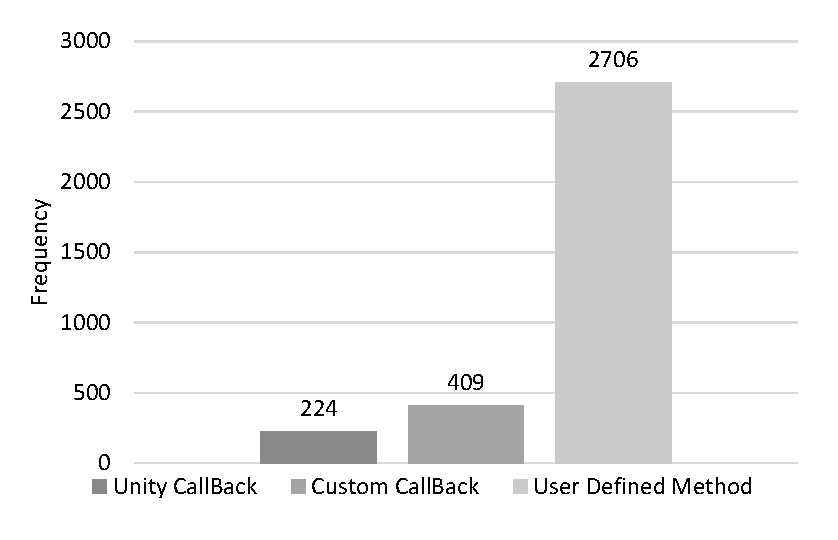
\includegraphics[width=0.8\textwidth]{figure/rq2_1.eps}
	%\vspace{-0.3cm}
	\caption{Type of Methods Prone to Performance Bug}
	%	\vspace{-0.3cm}	
	\label{figure:rq2methodtype}
\end{figure*}

Apart from that, we identified the top 10 frequently changed methods. If any method body is altered, we considered that the method is changed. As shown in the Figure~\ref{figure:rq2fixmethod}, Update method changes most frequently. Others are Start, Awake, OnEnable, etc. From the analysis, we identified that unity callbacks are related to performance bug locations. So, these methods are updated frequently. In this analysis, we did not consider callgraph dependency.

\begin{figure*}[t]
	%%\vspace{-0.2cm}
	\centering
	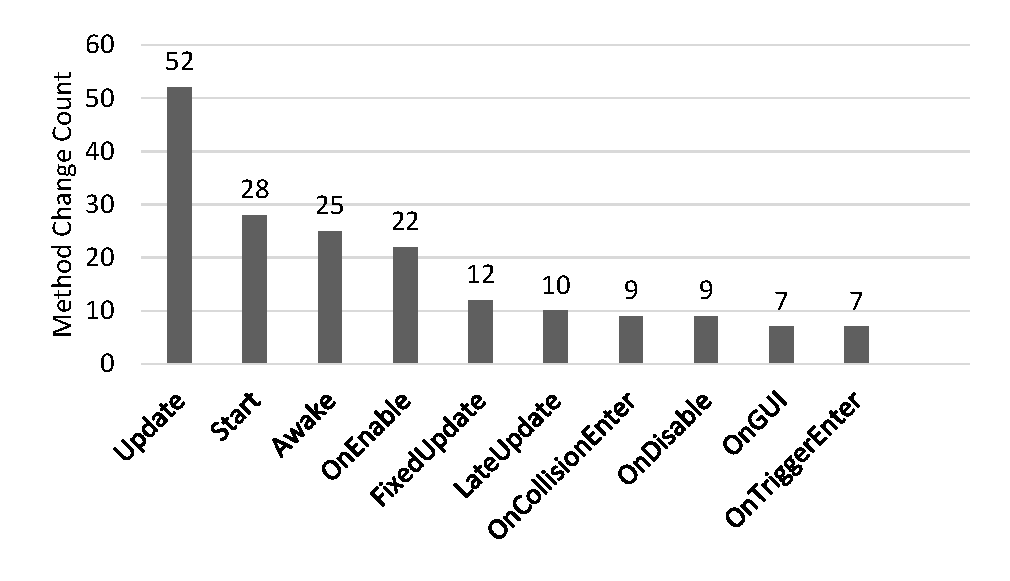
\includegraphics[width=0.8\textwidth]{figure/rq2_2.eps}
	%\vspace{-0.3cm}
	\caption{Fix Methods Without Considering Call Graph}
	%	\vspace{-0.3cm}	
	\label{figure:rq2fixmethod}
\end{figure*}


Later we did another analysis considering the code change method and static call graph dependency. According to the call graph figure, if a method is changed, then dependent methods are also considered as changed due to caller callee relationship. When we consider call graph dependency, we identified that the frequency of Unity callbacks also increased. That indicates that user-defined methods that are called from Unity callbacks are prone to performance bugs. Figure~\ref{figure:rq2fixmethodcallgraph} shows the frequency of Method change frequency based on code change and call graph dependency. 

\begin{figure*}[t]
	%%\vspace{-0.2cm}
	\centering
	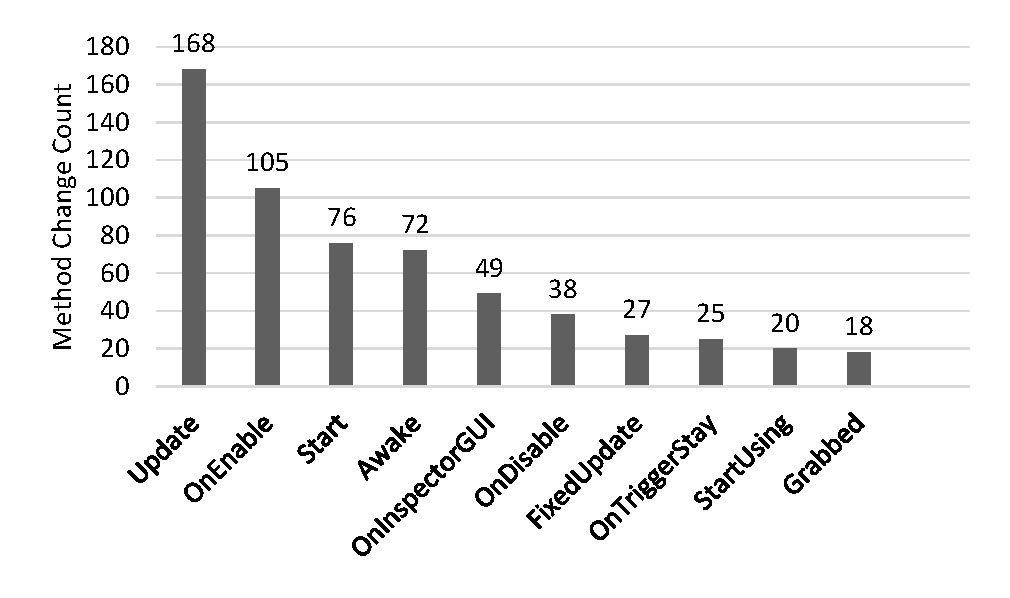
\includegraphics[width=0.8\textwidth]{figure/rq2_3.eps}
	%\vspace{-0.3cm}
	\caption{Fix Methods Considering Call Graph}
	%	\vspace{-0.3cm}	
	\label{figure:rq2fixmethodcallgraph}
\end{figure*}

If we consider distinct method changes contributed to 230 performance bugs, for 77 bugs, there is a change in the Update method; for 41 bugs, Start method is changed. OnInspectionGUI method changed in 39 bugs. Like other analyses, we also found the majority of the bugs fixes are related to callback methods. Figure~\ref{figure:rq2distinctmethod} shows the top 10 methods that contributed to performance bug fix.


\begin{figure*}[t]
	%%\vspace{-0.2cm}
	\centering
	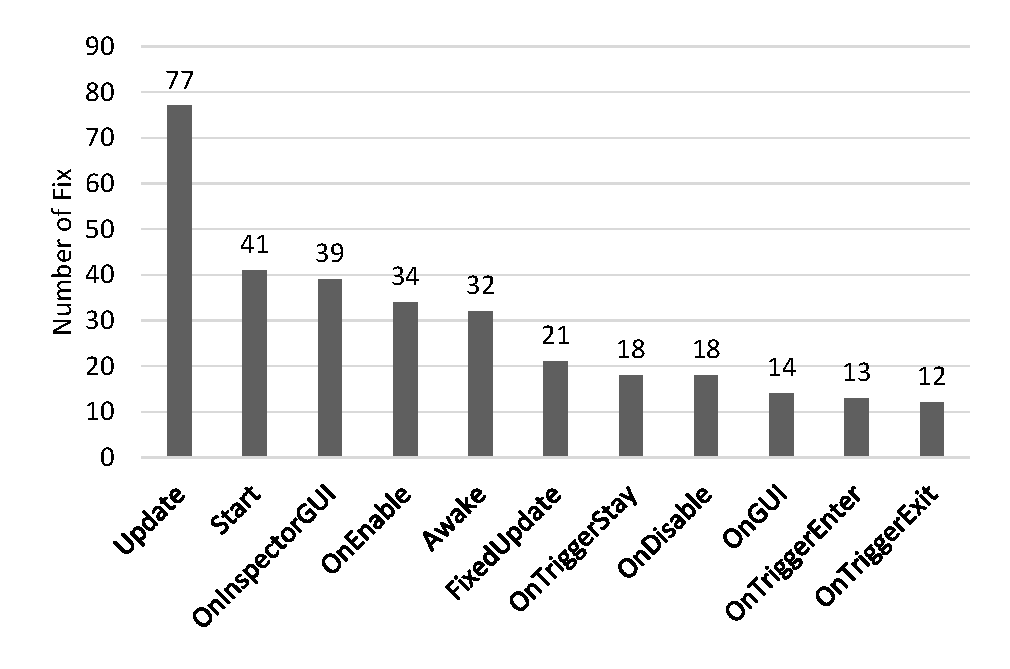
\includegraphics[width=0.8\textwidth]{figure/rq2_4.eps}
	%\vspace{-0.3cm}
	\caption{Individual Method Contribution to Fix Performance Bugs}
	%	\vspace{-0.3cm}	
	\label{figure:rq2distinctmethod}
\end{figure*}


\subsection{RQ3:Performance Fix Complexity}
\label{subsec:bugcomplexity}

Based on code change, we measured the Performance Fix Complexity. In terms of class change, the average class change per performance bug is 3.73, and the median is 1.00. For the case of MethodChange, the size average method change is 12.80 method, and the median is 3.50.  For statement change average statement change count is 32.83, and the median is 10.50. Figure~\ref{figure:rq2distinctmethod} shows the performance fix complexity distribution. From this analysis, we can confer that performance fixes are complex in nature.

\begin{figure*}[t]
	%%\vspace{-0.2cm}
	\centering
	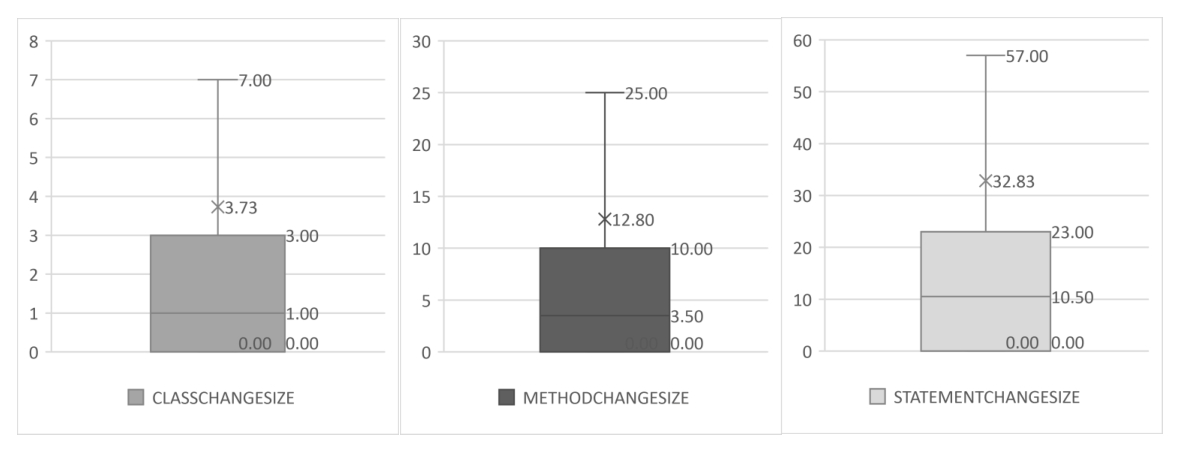
\includegraphics[width=0.9\textwidth]{figure/rq3_1.eps}
	%\vspace{-0.3cm}
	\caption{Performance Fix Complexity Distribution}
	%	\vspace{-0.3cm}	
	\label{figure:rq3}
\end{figure*}

Here some of the reasons why performance fixes are complex in nature. The most common reason is code and component dependency. So, if we change in one method or class, then in most cases, it's required to change in code dependency.  Another reason we observed that in many cases, developers fix several performance issues altogether.  For example, we found that when performing loop optimization, developers optimize loop related fixes in several locations. Two other reasons are lack of tool support and documentation. So, performance issues cannot be identified early. Later based on block or StackOverflow, developer refactors code. Since issues are identified later, code refactoring size becomes large.

\subsection{RQ4:Performance Bug Fix Location}
\label{subsec:bugcomplexity}
Based on the analysis of change(see Section~\ref{sec:commitanalysis}), here is the categorized result of performance bug fix location. As shown in Figure~\ref{figure:rq4}, 92 bugs are fixed by changing only in source code. Forty-five bugs require a change in unity asset or prefab file change. But 93 bugs required to change in both source and unity asset/prefab files. This is critical findings that, to improve or fix performance in many cases, we need to change asset/prefab files. So, the performance analysis of asset/prefab is also important.

\begin{figure*}[t]
	%%\vspace{-0.2cm}
	\centering
	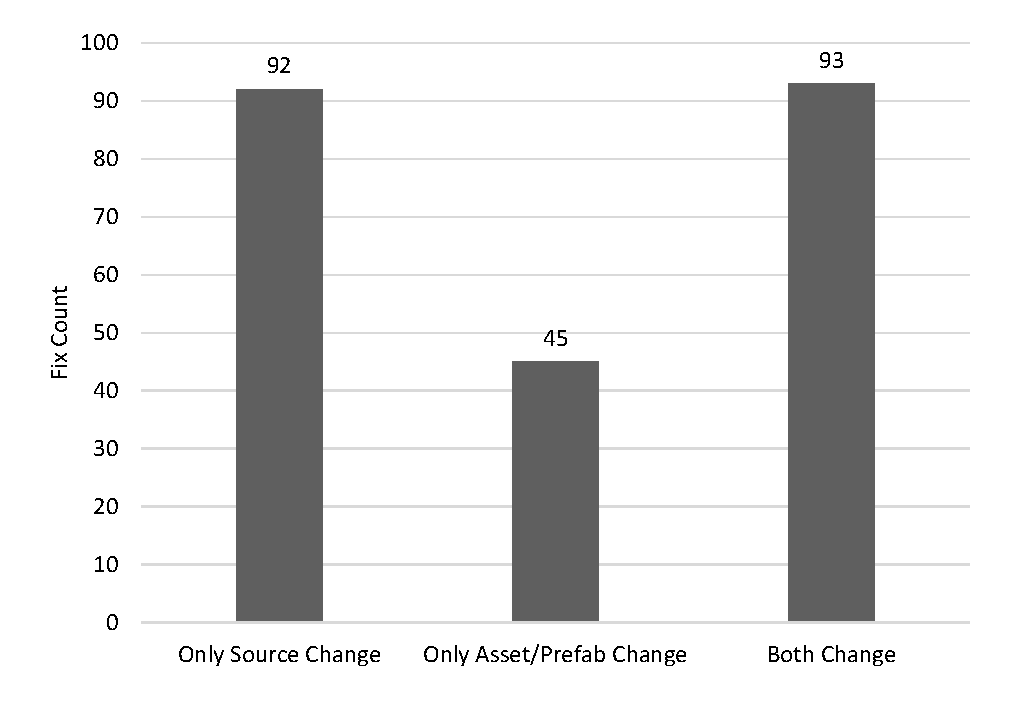
\includegraphics[width=0.9\textwidth]{figure/rq4_1.eps}
	%\vspace{-0.3cm}
	\caption{Performance Bug Location}
	%	\vspace{-0.3cm}	
	\label{figure:rq4}
\end{figure*}


\begin{example}
\begin{lstlisting}[escapechar=!]
!\hlp{-o.pos = mul(UNITY\_MATRIX\_MVP, v.vertex);}!
!\hlg{+o.pos = UnityObjectToClipPos(v.vertex);}!
\end{lstlisting}
  \caption{Example of Asset/Prefab Related Fix
  	\scriptsize{\textit{(RussellXie7/Unity\_Hololens\_Dev:b3823da)}}}
  \label{example:asset1}  
\end{example}

Example~\ref{example:asset1} shows such a performance fix where UnityObjectToClipPos routine is used to calculate Transformation of plane. Unity documentation also mentioned that mul routine could also be used for the Transform plane, but UnityObjectToClipPos is a more efficient way to calculate the plane.